% Standalone RAKL three-separations diagram (Paper I).
% access != coherence != authority : three independent planes, not a ladder.
% Build:  pdflatex three_separations.tex  -> three_separations.pdf
\documentclass[border=6pt]{standalone}
\usepackage{tikz}
\usepackage{helvet}\renewcommand{\familydefault}{\sfdefault}
\usetikzlibrary{positioning,arrows.meta,fit,backgrounds,calc}
\begin{document}
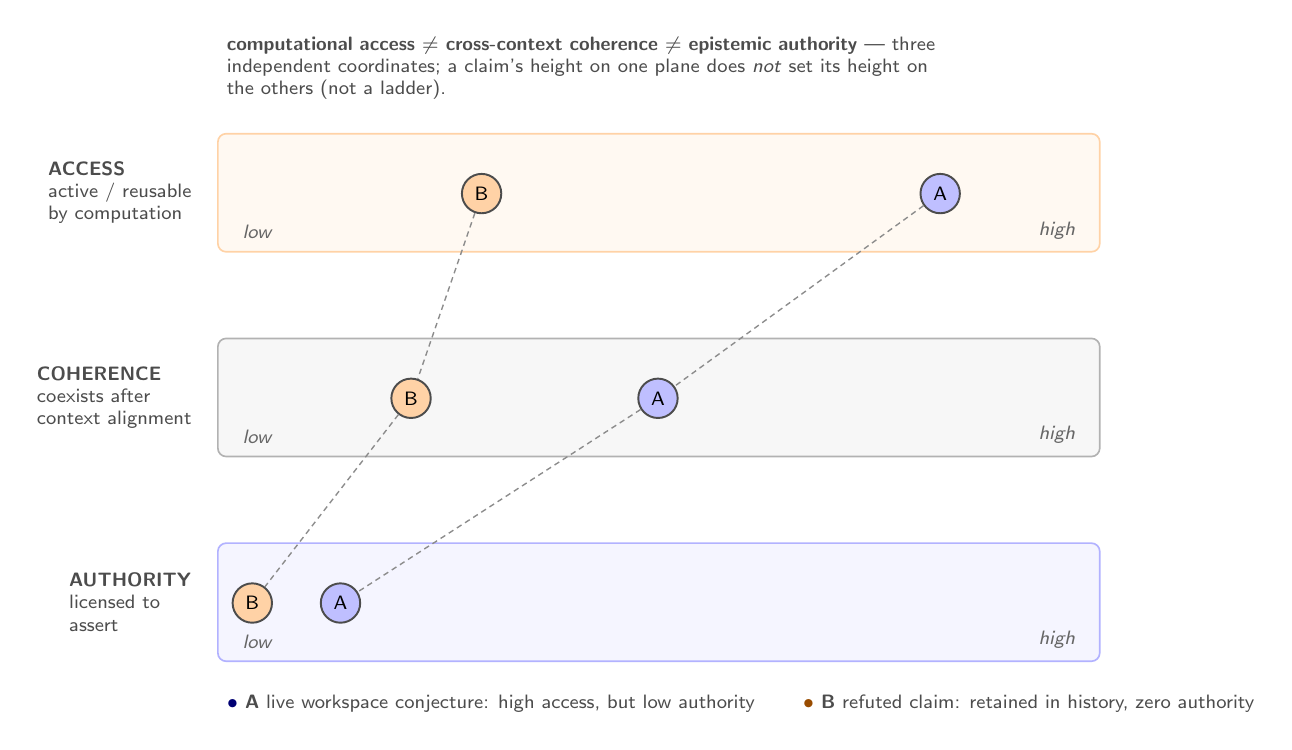
\begin{tikzpicture}[
  font=\small,
  >={Stealth[length=2.2mm]},
  plane/.style={rounded corners=3pt, draw=black!45, line width=0.6pt},
  capt/.style={align=left, font=\scriptsize, text=black!70},
  markA/.style={circle, draw=black!70, line width=0.7pt, fill=blue!25, minimum size=5mm, inner sep=0pt},
  markB/.style={circle, draw=black!70, line width=0.7pt, fill=orange!35, minimum size=5mm, inner sep=0pt},
  link/.style={-, line width=0.5pt, draw=black!45, dash pattern=on 2pt off 1.5pt},
  lbl/.style={font=\scriptsize\itshape, text=black!60},
]
\def\W{112}   % plane width in mm
\def\H{15}    % plane height in mm

% ---- three stacked horizontal planes ----
% y-baselines
\foreach \name/\y/\fill/\edge in {%
  authority/0/blue!4/blue!30,
  coherence/26/black!3/black!30,
  access/52/orange!5/orange!35}{
    \node[plane, fill=\fill, draw=\edge, minimum width=\W mm, minimum height=\H mm,
          anchor=south west] (\name) at (0,\y mm) {};
}
\node[capt, anchor=east] at ($(access.west)+(-2mm,0)$)
  {\textbf{ACCESS}\\active / reusable\\by computation};
\node[capt, anchor=east] at ($(coherence.west)+(-2mm,0)$)
  {\textbf{COHERENCE}\\coexists after\\context alignment};
\node[capt, anchor=east] at ($(authority.west)+(-2mm,0)$)
  {\textbf{AUTHORITY}\\licensed to\\assert};

% low/high axis hints on each plane
\foreach \name in {access,coherence,authority}{
  \node[lbl, anchor=south west] at ($(\name.south west)+(2mm,0.5mm)$){low};
  \node[lbl, anchor=south east] at ($(\name.south east)+(-2mm,0.5mm)$){high};
}

% ---- Claim A: live workspace conjecture -> high access, mid coherence, LOW authority ----
\node[markA] (Aacc) at ($(access.south west)+(0.82*\W mm,7.5mm)$) {\scriptsize A};
\node[markA] (Acoh) at ($(coherence.south west)+(0.50*\W mm,7.5mm)$) {\scriptsize A};
\node[markA] (Aaut) at ($(authority.south west)+(0.14*\W mm,7.5mm)$) {\scriptsize A};
\draw[link] (Aacc) -- (Acoh) -- (Aaut);

% ---- Claim B: refuted claim -> low access, low coherence, ZERO authority (retained in history) ----
\node[markB] (Bacc) at ($(access.south west)+(0.30*\W mm,7.5mm)$) {\scriptsize B};
\node[markB] (Bcoh) at ($(coherence.south west)+(0.22*\W mm,7.5mm)$) {\scriptsize B};
\node[markB] (Baut) at ($(authority.south west)+(0.04*\W mm,7.5mm)$) {\scriptsize B};
\draw[link] (Bacc) -- (Bcoh) -- (Baut);

% ---- legend for the two example claims ----
\node[capt, anchor=north west] at ($(authority.south west)+(0,-3mm)$)
  {{\color{blue!45!black}$\bullet$}~\textbf{A} live workspace conjecture: high access, but low authority \qquad
   {\color{orange!60!black}$\bullet$}~\textbf{B} refuted claim: retained in history, zero authority};

% ---- "not a ladder" message ----
\node[capt, anchor=south west, text width=90mm] at ($(access.north west)+(0,3mm)$)
  {\textbf{computational access} $\neq$ \textbf{cross-context coherence} $\neq$ \textbf{epistemic authority}
   --- three independent coordinates; a claim's height on one plane does \emph{not} set its height on the others (not a ladder).};
\end{tikzpicture}
\end{document}
